\documentclass[
  % LuaLaTeXを使う
  luatex,
  % 用紙サイズをA4にする
  paper=a4paper,
  % 欧文のフォントサイズを11ptにする
  fontsize=11pt,
  % レポート形式
  report,
  % 日本語組版処理の記述と矛盾する設定がある場合に通知
  jlreq_notes,
]{jlreq}

\usepackage{fontspec}
\usepackage[framemethod=tikz]{mdframed}
\usepackage{enumitem}
\usepackage{tocloft}  % 目次のカスタマイズ用パッケージ
\usepackage{geometry}  % ページレイアウトの調整
% jlreqsetupで色々設定できるようにする
\usepackage{jlreq-complements}
% 画像を扱う
\usepackage{graphicx}
% pdfのハイパーリンクを設定
\usepackage[hidelinks]{hyperref}
% 相対パスでファイルを読み込む
\usepackage{import}
% 枠をつける
\usepackage{ascmac}  
% 章やページの合計を扱う
\usepackage{totcount}
% svgを扱う
\usepackage{svg}
% 表の罫線を扱う
\usepackage{booktabs}
% 数式関連
\usepackage{amsmath,amssymb}
\usepackage{mathtools}
\usepackage[
  % mathtoolsと一部競合するため,警告を無視
  warnings-off={mathtools-colon,mathtools-overbracket}
]{unicode-math}
\unimathsetup{math-style=TeX,bold-style=TeX}
\setmainfont[Ligatures=TeX]{Latin Modern Roman}
\setsansfont[Ligatures=TeX]{Latin Modern Sans}
\setmonofont{Latin Modern Mono}
\setmathfont{Latin Modern Math}
% 目次の章タイトルを太字にする
\renewcommand{\cftchapfont}{\bfseries}  % 章タイトルを太字にする

% フォントを設定
% unicode-mathの後でないとフォントが変更されない
\usepackage[
  % 多ウェイト化を有効にする
  deluxe,
  % jlreqで使えるようにする
  jfm_yoko=jlreq,
  jfm_tate=jlreqv,
]{luatexja-preset}

% jlreqの設定
\jlreqsetup{
  % 参考文献の見出しの出力命令を設定
  thebibliography_heading={
    % 見出しを章にする
    \chapter*{\refname}
    \renewcommand{\cftsecfont}{\normalfont}  % 節タイトルを通常フォント
    % 目次に追加
    \addcontentsline{toc}{chapter}{\refname}
  },
}

\geometry{top=40mm, bottom=30mm, left=25mm, right=25mm}



\begin{document}

\begin{titlepage}
  \centering

  {\Large
    岐阜大学工学部 \\ [0.5em]
    電気電子・情報工学科 \\ [0.5em]
    令和6年度卒業論文 \\
  } 
  \vspace{8em} 

  {\huge
    セキュアなV2Vアドホックネットワーク \\
    ルーティングプロトコルのための \\
    EdDSA署名方式の評価 \\
  }
  \vspace{12em}

  \LARGE 三嶋研究室 \\ [1em]
  \Large 学籍番号:1213033107 \\ 
  \huge 永野 正剛 \\ [1em]
  \LARGE 指導教員:三嶋 美和子 教授 \\

  \vfill 
\end{titlepage}
% 最初のページはページ番号をローマ数字にする
\pagenumbering{roman}

% 目次を表示
\tableofcontents

\clearpage
% ページ番号を元に戻す
\pagenumbering{arabic}

\chapter*{はじめに}
\addcontentsline{toc}{chapter}{はじめに}  % 目次に追加
\chapter[   準備]{準備}
\section{\textbf{VANET}}
\textbf{VANET(Vehicle Ad Hoc Network)}とは, モバイル
アドホックネットワーク技術を車両間通信に応用したネットワークである. 
\cite{adhoc, vanet} 車両間の通信(Vehicle-to-Vehicle, V2V), および
車両とインフラ(路側機やドローン)間通信(Vehicle-to-Infrastructure, V2I)\cite{drone}で
構成され, 固定されたインフラストラクチャに依存せず, ノード同士が
自律的に通信ネットワークを形成する. VANETでは, 車両間の通信距離が
無線通信の範囲を超えることが一般的であるため, 図1.1のように, 
データを送信元から宛先まで直接通信できない場合に, 
中継ノードを経由してデータを転送する. このような通信を
\textbf{マルチホップ通信}という.\\


{\Huge 図1.1を挿入}\\

VANETには次の5つの特徴がある.\\[0.5em]
\noindent\textbf{(1) 十分な電力供給}\\
\indent 車両はエンジンによって継続的に電力が供給されるため, 
スマートフォンのような電池駆動のモバイルデバイスに比べて電力の制約を
ほとんど受けない. これより, 長時間の稼働や高い通信レートの実現が
可能である. しかし, 高性能な通信モジュールやセンサーを多数搭載する場合, 
車両の燃費やエネルギー効率に影響を与える可能性があるとして, 
効率的なデバイス設計が必要である.\\[1em]
\noindent\textbf{(2) 自身の位置情報}\\
\indent 車両はGPSを搭載しているため,  自身の位置情報を取得できる.\\[1em]
\noindent\textbf{(3) ネットワークトポロジーの急速な変化}\\
\indent 無線通信では,ノード同士が直接的に通信可能であることを
接続しているといい, この接続状態を基にネットワーク全体の構造が形成される.
そして, このネットワーク構造をネットワークトポロジーという. 
VANETでは通信するノードを車両と想定しているため, 
移動速度の速いノードが動的にネットワークを形成する. 
そのため, 接続の頻繁な確立と切断が発生し, 
ネットワークトポロジーは急速に変化する. \\[1em]
\noindent\textbf{(4) 移動パターン}\\
\indent 車両の動きは道路や建造物などの物理的構造に従う.\\[1em]
\noindent\textbf{(5) 安全に関する情報のリアルタイム性}\\
\indent 交通事故や道路状況に関する情報を即座に共有するためには 
低遅延かつ信頼性の高い通信が求められる.\\

VANETには, 車両間通信や車両とインフラ間通信を実現するための
優れた技術としてのポテンシャルがある一方で, 
いくつかの課題も抱えている.
その中でも, セキュリティに関する課題はVANETを安全かつ信頼性の
高いシステムとして運用する上で最も重要な問題の一つとなっている.
\cite{vanet-challenge,vanet-security}\\


\section{\textbf{GPSR}}
\textbf{GPSR(Greedy Perimeter Stateless Routing)}\cite{gpsr}は, 
位置情報を利用してパケットを転送する位置ベースの
ルーティングプロトコルであり, VANETのような動的で高速に変化する
ネットワーク環境に適している.
GPSRでは, 自身の位置やIPアドレスなどの情報をのせたHelloパケットを
一定間隔で隣接ノードに送信する.
図1.2に示すように, それぞれのノードはIPアドレスや隣接ノードの
位置などの情報が記載された隣接ノードテーブルをもち, 
受信したHelloパケットの情報を用いて隣接ノードテーブルを
更新することにより周辺ノードの情報を把握する. 
この隣接ノードテーブルの情報を基に, Greedy Forwarding と 
Perimeter Forwarding を組み合わせたルーティングプロトコルを行う.\\

{\Huge 隣接ノードデーブルの図1.2を挿入}\\

\noindent {\Large\textbf{Greedy Forwarding}}\\
\indent \textbf{Greedy Forwarding}はGPSRの基本的な
ルーティングプロトコルである. 図\ref{fig:greedy}に示すように, 
送信ノードSは, 宛先ノードDの位置情報をもとに
自身の電波伝搬範囲内のノードから, Dに最も近いノードを
ネクストホップとして選択する. 前提として, 送信ノードSは宛先ノードDの
位置情報を事前に把握しているものとする. 点線で書かれた円は全ノードの
受信感度が等しい場合の送信ノードSの電波伝搬範囲を, 
破線は宛先ノードとの距離を表している.

\begin{figure}
  \centering
  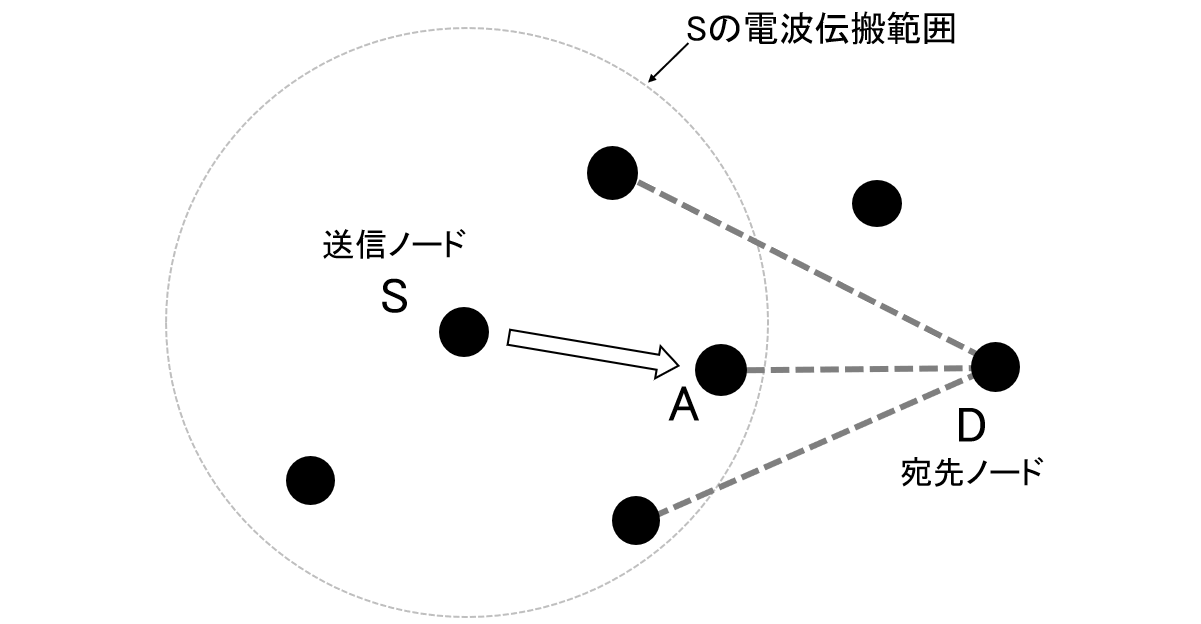
\includegraphics[scale=0.55]{figures/greedy.png}
  \caption{Greedy Forwarding\cite{shinato}}
  \label{fig:greedy}
\end{figure}

Greedy Forwardingでは局所最大問題と呼ばれる問題が生じてしまうことがある. 
\textbf{局所最大問題}とは, 図\ref{fig:local}に示すように, 送信ノードSの電波伝搬範囲内に
宛先ノードDが存在しない, かつ, 送信ノードSが自身の
電波伝搬範囲内で宛先ノードDに最も近い場合, 選択できる
ネクストホップが存在しなくなるという問題である.

\begin{figure}
  \centering
  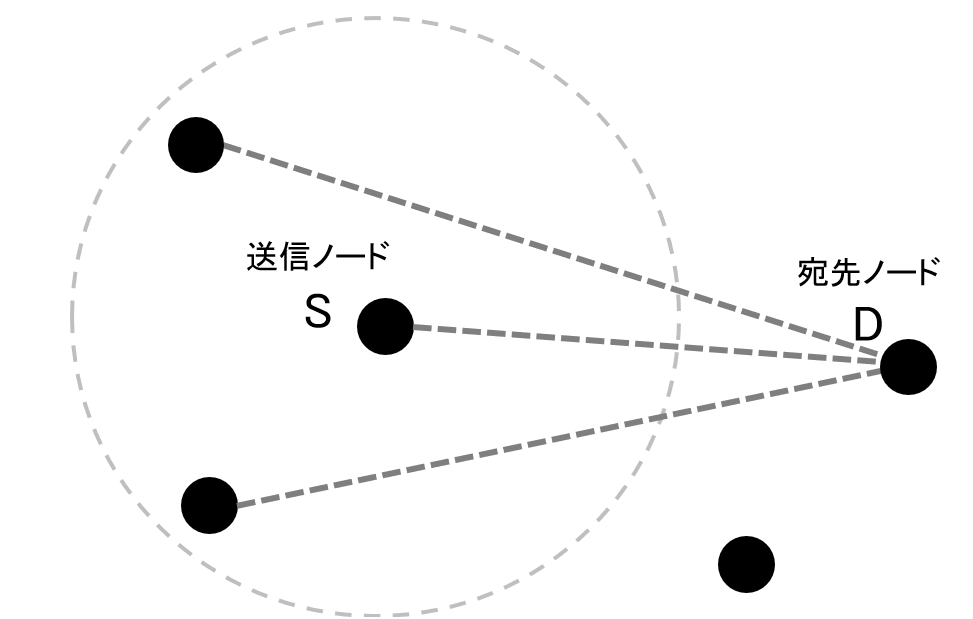
\includegraphics[scale=0.55]{figures/local.png}
  \caption{局所最大問題}
  \label{fig:local}
\end{figure}

\noindent {\Large\textbf{Perimeter Forwarding}}\\
Greedy Forwardingで局所最大問題が発生した場合に, 
Perimeter Forwardingが使用される. 
図1.5のように, 送信ノードSを中心に
\textbf{Right Hand Rule} に則って反時計回りにノードを探索し, 
最初に発見したノードをホップとして選択する方式である.

\textbf{図1.5を挿入}
\section{\textbf{楕円曲線}}
\subsection{EdDSA}
\section{\textbf{デジタル署名}}
\textbf{デジタル署名}とは, 公開鍵暗号の仕組みを利用して作られた暗号技術であり, 
電子文書やメッセージの真正性と完全性を検証するために使用される. 
この技術は, データの信頼性を確保し, かつ, 送信者がデータの送信を否定できない
非否認性を提供する.\\
% \textbf{デジタル署名}とは, するための
% 暗号技術であり, 電子データの送信者を認証するとともに, 
% そのデータが通信途中で改ざんされていないことを保証する仕組みである. 
% この技術は, データの信頼性を確保し, 送信者がデータの送信を否定できない
% 非否認性を提供する.\\
\indent 一般に, デジタル署名は以下の3つのフェーズから構成される.

\begin{enumerate}
  \item \textbf{鍵生成}\\
  \indent 署名者(送信者)が署名に使用する鍵のペア, 
  すなわち検証鍵(公開鍵)と署名鍵(秘密鍵)を生成するフェーズである. 
  署名鍵は署名者が厳重に管理し, 秘密に保管する. 一方, 検証鍵は
  受信者や第三者に公開され, 署名の検証に用いられる.
  \item \textbf{署名生成}\\
  \indent メッセージ作成者(送信者)は, 署名対象のメッセージから
  ハッシュ関数を用いてハッシュ値を計算する. このハッシュ値は, 
  メッセージがわずかでも変更されると全く異なる値となるため, 
  メッセージが改ざんされていないこと(完全性)を検証するための
  重要な要素である. 続いて, メッセージ作成者は自身の署名鍵(秘密鍵)を
  使ってハッシュ値に署名を行う. 署名鍵がメッセージ作成者
  しか保持していないことと, メッセージ作成者以外が署名鍵を求めることは
  計算量的に困難なことから, 署名はメッセージの作成者が正当であること
  (真正性)を証明する役割を果たす. 
  \item \textbf{署名検証}\\
  \indent 検証者(受信者)は, 署名者が公開した検証鍵(公開鍵)を用いて
  署名を検証する. この検証プロセスにより, 署名が署名鍵と対になる
  検証鍵によって生成されたことを確認できるため, メッセージが正規の
  作成者によって署名され, 送信後に改ざんされていないことが保証される.
\end{enumerate}

デジタル署名にはさまざまなアルゴリズムが存在する. その中でも,    
\textbf{国立標準技術研究所(National Institute of Standards and Technology, NIST)}
による情報処理標準規格 FIPS に基づいて設計された
\textbf{ECDSA(Elliptic Curve Digital Signature Algorithm)}は, 
V2V通信のようなリアルタイム性やリソース制約が求められる環境に
適しているため, 先行研究\cite{shinato}で使用されていた. 
したがって, 本研究でも, ECDSA方式を用いて
シミュレーション実験をし, EdDSAと比較評価を行う. \\
以下に, ECDSAの概要を示す. \\[1em] 


% \noindent {\Large\textbf{DSA}}\\
% \textbf{DSA (Digital Signature Algorithm)}は, 1993 年に FIPS 186-4として
標準化された, DSS (Digital Signature Standard) の主要なアルゴリズムの
1つであった. なお, 2023 年の FIPS 186-5\cite{fips186-5} では,DSAは
新たにデジタル署名を行うことには推奨されないが, 標準策定以前に行われた
署名の検証には引き続き利用可能とされている.\\
\indent DSAの3つのフェーズにおける処理は以下の通りである.\\[0.5em]
\let\ltxlist\list
\begin{breakitembox}[l]{\textbf{鍵生成}}
   
  \begin{enumerate}[parsep=7pt]
    \item セキュリティパラメータとして整数 $L,N (L>N)$ を定める. 
    FIPS186-4では以下の4つの値の組が規定されている.
    \begin{center}
      $(L,N) = (1024,160), (2048,224), (2048,256), (3072,256)$
    \end{center}
    \item $N$ビットのランダムな素数$q(2^{N-1}<q<2^{N})$, 
    $L$ ビットのランダムな素数$p(2^{L-1}<q<2^{L})$ を選ぶ.
    ただし, $q$は$p-1$を割り切る素数とする.
    \item ランダムな整数$a<p-1$に対し,
    \[
      g\equiv a^{\frac{p-1}{q}}\pmod p
    \] 
    を計算する. ただし,$g=1$である場合は再度$a$を選び直す.
    \item ランダムな整数$x(1<x<q)$に対し,
    \[begin{equation}]
      y\equiv g^x\pmod p
    \]
    を計算する.
    \item $p,q,g$は専用のパラメータとして, $y$は検証鍵(公開鍵)として
    公開する. $x$は署名鍵(秘密鍵)として安全に管理する.
  \end{enumerate}
\end{breakitembox}
\vspace{1em}
\indent 任意長のメッセージ $M$ に対して, パラメータ$p, q, g$, 秘密鍵$x$, 
ハッシュ関数$H$ を用いて, 次のように署名を生成する.
\vspace{1em}
\let\ltxlist\list
\begin{breakitembox}[l]{\textbf{署名生成}}
   
  \begin{enumerate}[parsep=7pt]
    \item ランダムな整数 $k(1<k<q)$ を選ぶ.
    \item $r\equiv (g^k\pmod p)\pmod q$ を計算する. 
    ただし, $r=0$ の場合は再度 $k$ を選び直す.
    \item $s\equiv k^{-1}(H(M+xr))\pmod q$ を計算する.
    ただし, $s=0$ の場合は再度 $k$ を選び直す.
    \item $(r,s)$ をメッセージ$M$に対する署名とし, 
    $M$とともに受信者に送信する.
  \end{enumerate}
\end{breakitembox}
\vspace{1em}
メッセージ$M$に対する署名$(r, s)$を検証するには, パラメータ$(p,q,g)$, 
公開鍵$y$, ハッシュ関数$H$を用いて, 以下のアルゴリズムを実行する.
\vspace{1em}
\let\ltxlist\list
\begin{breakitembox}[l]{\textbf{署名検証}}
   
  \begin{enumerate}[parsep=7pt]
    \item 受け取った$(r,s)から, $$0<r<q$ かつ $0<s<q$ であることを確認する. 
    これを満たさない場合は署名を棄却する.
    \item $w\equiv s^{-1}\pmod q$ を計算する.
    \item $u_1\equiv wH(M)\pmod q$を計算する.
    \item $u_2\equiv rw\pmod q$ を計算する.
    \item $v\equiv (g^{u_1}y^{u_2}\pmod p)\pmod q$ を計算する.
    \item $v=r\pmod  q$ であれば, 署名を受理する. そうでなければ
    不正な署名とみなし, 棄却する.
  \end{enumerate}
\end{breakitembox}
\vspace{1em}
\indent 正当なメッセージと署名の組$(M, (r, s))$に対し, 
\[
  g^{u_1}y^{u_2}\equiv g^{u_1+xu_2} \equiv g^{H(M)+xr}w\equiv g^{k}\pmod p
\]
が成り立つ. これは 
\begin{align*}
  v &\equiv (g^{u_1}y^{u_2} \mod p) \mod q \\
    &\equiv (g^k \mod p) \mod q \\
    &\equiv r \mod q
\end{align*}
であることを示す.\\
\indent ここで, メッセージや署名に対し改ざんが行われたとしよう. 
攻撃者が, 署名検証条件 $v \equiv r \pmod{q}$ を
満たすように操作できた場合, その攻撃は成功したとみなされる. ただし, 
署名生成に使用される値には, 署名者しか知らない秘密の乱数$k$が
含まれており, この$k$は離散対数問題に基づいて計算されるため, 
十分なビット長を持つ$p$および$q$の下では, 改ざんを成功させることは
計算量的に極めて困難である.さらに, 署名生成プロセスではメッセージの
ハッシュ値$H(M)$が使用されており, このハッシュ値はハッシュ関数の
衝突困難性に依存している. したがって, 攻撃者が異なるメッセージ $M'$ を
生成し, そのハッシュ値が元のメッセージ $M$ と同じ $H(M') = H(M)$ と
なるようにすることも困難である. この性質により, 改ざんされたメッセージ
$M'$のハッシュ値は$H(M')\neq H(M)$となり, 
署名検証条件 $v \equiv r \pmod{q}$ が成立しなくなる.
また, 攻撃者がメッセージ$M$をそのままにして署名$(r, s)$を
改ざんした場合でも, 署名にはハッシュ値$H(M)$が埋め込まれているため, 
署名検証条件は満たされない. この結果, 署名検証アルゴリズムの最終段階で
署名が有効と判定される場合, 署名$(r, s)$もメッセージ$M$も
改ざんされていないことが保証される.



\noindent {\Large\textbf{ECDSA}}\\
\indent \textbf{ECDSA (Elliptic Digital Signature Algorithm)}は, 
DSA\cite{fips186-5}を楕円曲線暗号(Elliptic Curve Cryptography, ECC)を基盤として
改良したデジタル署名アルゴリズムである.
ECDSAは, 2000年に FIPS 186-2として標準化され, 
最新版であるFIPS 186-5\cite{fips186-5}でも採用されている.
ECDSAは, DSAよりも短い鍵長で同等の安全性を確保できるため, 
計算量が少なく, 低性能なデバイスでも高速な処理が可能であり, 
かつ演算規則の複雑さから攻撃者が鍵を推測することも困難である. \\
\indent この項では, ECDSAの理解に必要となる楕円曲線とその上での演算について
説明し, その後, ECDSAのアルゴリズムについて述べる.\\[1em]

\noindent{\large\textbf{楕円曲線}}\\
\indent 体$\mathbb{F}_p$($p$は素数)上で定義された楕円曲線とは以下の式で与えられる
代数曲線である.
\[
  y^2+a_1y+a_3y=x^3+a_2x^2+a_4x+a_6  (a_1,a_2,a_3,a_4,a_6\in\mathbb{F}_p)
\]
この式をWeierstrass方程式という\cite{安田}. 
特に, $p\neq 2,3$の場合, 以下の標準形に簡略化できることが知られている. 
\begin{equation}\label{weierstrass}
  y^2=x^3+ax+b  (a,b\in\mathbb{F}_p)
\end{equation}
\indent 楕円曲線(式(\ref{weierstrass}))の判別式$\Delta$が
\[
  \Delta=-16(4a^3+27b^2)\neq 0
\]
を満たすとき, 楕円曲線(式\ref{weierstrass})は\textbf{非特異}であるという. 
非特異である楕円曲線は, 尖点や自己交差点, 孤立点を持たないため, 
楕円曲線が非特異であることは, 後述する楕円曲線上の点に対する演算
(加算やスカラー倍)が矛盾なく定義されるために必要不可欠である.\\
\indent 楕円曲線上の点$P=(x,y)$のうち$x,y$がともに有限体
$\mathbb{F}_p$の元であるものを\textbf{有理点}という. また, 楕円曲線上には
\textbf{無限遠点}と呼ばれる特殊な点$\mathcal{O}$の存在を仮定し, これも楕円曲線上の
有理点の集合に含める. 有理点の集合は, 以下で述べる演算に関して
群の構造をもつ. 楕円曲線暗号方式では,この性質が利用される.\\[1em]
\noindent\textbf{楕円曲線上の点の加算}\\
\indent 楕円曲線上の点$P=(x_1,y_1)$と$Q=(x_2,y_2)$の加算 $P+Q$ を
以下のように定義する.
\begin{enumerate}
  \item[(i) ] 2点$P,Q$を通る直線が$y$軸と平行でない場合%(図1.6):
  \begin{enumerate}
    \item[1. ] 点$P,Q$を通る直線$L$を引く.
    \[
      L : y-y_1 = \frac{y_2-y_1}{x_2-x_1}(x-x_1)
    \]
    \item[2. ] $L$と楕円曲線$E$の交点を$R(x_3,y_3)$とする.
    \[
    \begin{aligned}
      x_3 &= \left(\frac{y_2-y_1}{x_2-x_1}\right)^2-x_1-x_2\\
      y_3 &= \frac{y_2-y_1}{x_2-x_1}(x_1-x_3)-y_1
    \end{aligned}
    \]
    \item[3. ] $R$の$x$軸対称な点$R'(x_3,-y_3)$が$P+Q$となる.
    \[
      P+Q=R'
    \]
  \end{enumerate}
  % {\LARGE\textbf{図1.6を挿入}}\\
  \item[(ii) ] 2点$P,Q$を通る直線$L$が$y$軸と平行である場合:\\
  \indent この場合, 直線$L$は2点$P,Q$以外で楕円曲線$E$と交わらない.\\ 
  \indent 無限遠点$\mathcal{O}$が$P+Q$となる.
  \[
    P+Q=\mathcal{O}
  \]
  \item[(iii) ] 2点$P,Q$が同一の点である場合%(図1.7):\\
  \begin{enumerate}
    \item[1. ] 点$P$における接線$L'$を引く. 
    \[
      L' : y-y_1 = \frac{3x_1^2 + a}{2y_1}(x - x_1)
    \] 
    \item[2. ] $L'$と楕円曲線$E$の交点を$R(x_3,y_3)$とする.
    \[
    \begin{aligned}
      x_3 &= \left(\frac{3x_1^2 + a}{2y_1}\right)^2-2x_1\\
      y_3 &= \frac{3x_1^2 + a}{2y_1}(x_1-x_3)-y_1
    \end{aligned}
    \]
    \item[3. ] $R$の$x$軸対称な点$R'(x_3,-y_3)$が$P+Q$となる.
    \[
      P+Q=2P=R'
    \]
  \end{enumerate}
  % {\Huge\textbf{図1.7を挿入}}
  \item[(iv) ] $P=\mathcal{O}$または$Q=\mathcal{O}$である場合:\\
  \indent 無限遠点は加算において加法単位元の役割を果たす.
  \[
  \begin{aligned}
    P+\mathcal{O}&=P\\
    \mathcal{O}+Q&=Q
  \end{aligned}
  \]    
\end{enumerate}
\vspace{0.5em}
\noindent\textbf{スカラー倍算}\\
\indent 正整数$k$による点$G$のスカラー倍$P=kG$は, 点$G$を$k$回加算した結果を表す.
\[
  P=kG=\underbrace{G+G+\cdots+G}_{k\text{回}}
\]
\indent ある基準点$G$に対し, $P = kG$となる楕円曲線上の点$P$が与えられたとき, 
$k$と$G$から$P$を求めるのは容易である. しかし, 逆に$G$と$P$から$k$を
求めるのは計算量的に困難であることが知られている. 
これを\textbf{楕円曲線上の離散対数問題(Elliptic Curve Discrete Logarithm Problem, ECDLP)}という.\\[1em]

\noindent{\large\textbf{ECDSAのアルゴリズム}}\\
\indent ECDSAの3つのフェーズにおける処理は以下の通りである.
\vspace{1em}
\let\ltxlist\list
\begin{breakitembox}[l]{\textbf{鍵生成}}
   
  \begin{enumerate}[parsep=7pt]
    \item 法となる素数$p$と, 楕円曲線$E$を選び, $E$上の基準点$G$を選ぶ.
    \item $d$を$2\leq d\leq n-1$の範囲からランダムに選び, 
    署名鍵(秘密鍵)として安全に管理する. ただし, $n$は$G$の位数である.
    \item $Q=dG$を計算し, $Q$を検証鍵(公開鍵)とする.
  \end{enumerate}
\end{breakitembox}
\vspace{1em}
\let\ltxlist\list
\begin{breakitembox}[l]{\textbf{署名生成}}
   
  \begin{enumerate}[parsep=7pt]
    \item $k$を$2\leq k\leq n-1$の範囲からランダムに選び, $kG$の
    $x$座標を$r$とする.
    \item メッセージ$M$に対し, ハッシュ関数$H$を用いて, $h=H(M)$を計算する.
    \item $s\equiv k^{-1}(h+dr)\pmod n$を計算する.
    \item $(r,s)$をメッセージ$M$に対する署名とし, 
    $M$とともに受信者に送信する.
  \end{enumerate}
\end{breakitembox}
\vspace{1em}
\let\ltxlist\list
\begin{breakitembox}[l]{\textbf{署名検証}}
   
  \begin{enumerate}[parsep=7pt]
    \item $(M,(r,s))$を受け取り, $h=H(M)$を計算する. 
    \item $u\equiv s^{-1}h\pmod n$, $v\equiv s^{-1}r\pmod n$を計算する.
    \item 楕円曲線上の点として, 
    \[
      Q'=(x',y')=uG+vQ
    \]
    を計算する.
    \item $Q'$の$x$座標$x'$が$r$と一致すれば, 署名を受理する.
    そうでなければ不正な署名とみなし, 棄却する.
  \end{enumerate}
\end{breakitembox}
\vspace{1em}
\indent 正当なメッセージと署名の組$(M, (r, s))$に対し, 
\begin{align*}
  Q'  &= uG + vQ\\
      &= s^{-1}hG + s^{-1}rQ \\
      &= s^{-1}hG + s^{-1}rdG \\
      &= s^{-1}hG + s^{-1}(sk-h)G \\
      &= s^{-1}(hG + skG - hG) \\
      &= s^{-1}skG \\
      &= kG
\end{align*}
が成り立つため, $Q'$の$x$座標が$r$と一致するかどうかを確認することで
署名検証が可能である.\\

\chapter[   EdDSA]{EdDSA}
\section{データの変換}
EdDSAのアルゴリズム内では, 整数や点をオクテット列に変換するエンコードと
その逆変換であるデコードが行われる\cite{インフォーズ}.\\
 以下にEd25519で使用されるデータの変換について説明する.\\
なお, $b$は8の倍数とする. 
また, 16進数表記の数値は$0x$FFのようにその数値の前に
「$0x$」を付けることで表す.\\[1em]

\noindent{\large\textbf{ビット列}}\\
 8ビットからなるビット列
\[
b_0b_1b_2b_3b_4b_5b_6b_7
\]
を\textbf{オクテット}と呼ぶ.
厳密には8ビット以外を指すこともある「バイト」の代わりに, 
必ず8ビットのことを指すものとして使われている語である.\\
ここで, 最下位ビットは$b_0$, 最上位ビットは$b_7$である.\\
\indent 例として, $0x12$は, 2進数では$00010010$であり, 
8ビットのビット列で表すと$01001000$となる.\\ 

\noindent{\large\textbf{リトルエンディアン形式}}\\
 リトルエンディアン形式とは, 数値をバイト単位で格納する際に, 
最下位バイト(数値の最小の値を持つバイト)を先頭に配置し, 
続けてその次に小さいバイトを配置していく方法を指す.
これは, 通常の十進法で右端から左へ数字を読むのと逆の順番で
データを並べることになる.\\
 例えば, 32ビットの $0x12345678$ をリトルエンディアン形式で
メモリに格納すると, 次のような順番でバイトが並ぶ:
\begin{itemize}
  \item 最下位バイト(1バイト目):$0x78$
  \item 2バイト目:$0x56$
  \item 3バイト目:$0x34$
  \item 最上位バイト(4バイト目):$0x12$
\end{itemize}
\noindent このようにして, $0x12345678$ はメモリ上で 
$0x78, 0x56, 0x34, 0x12$ の順番に格納される.\\[1em]

\noindent{\large\textbf{エンコードとデコード}}
\begin{enumerate}
  \item ENC$(s)$\\
   整数をオクテット列に変換し, データとして扱いやすくするための関数.\\
  処理:\\
   $b$ビットの整数$s$を入力として, $s$を リトルエンディアン形式にして
  $\tfrac{b}{8}$個のオクテットに変換して出力する.
  \item DEC$(t)$\\
   計算で使用できるよう, オクテット列を元の整数に戻す関数.\\
  処理:\\
   オクテット列$t$を入力として, 整数$s$に変換して出力する.
  つまり, $\mathrm{DEC}(t)=\mathrm{ENC}^{-1}(t)=s$である.
  \item ENCE$(A)$\\
   ツイストエドワーズ曲線上の点をオクテット列に変換し, 
  $x$座標の符号も付加して効率的に表現するための関数.\\
  処理:\\
   はじめに符号関数を
  \[
    \text{sign}(a) =
    \begin{cases}
    0 & \text{if } a \geq 0 \\
    1 & \text{if } a < 0
    \end{cases}
  \]
  とする.ここで$a$は整数である.\\
   ツイストエドワーズ曲線上の点A$(x,y)$の$y$を入力として, 
  ENC$(y)$によりオクテット列$y'=(y'_1,y'_2,...,y'_\frac{b}{8})$に変換し, 
  $y'_\frac{b}{8}$の最上位ビットにsign$(x)$を格納した
  オクテット列を出力する.
  \item DECE$(t)$\\
   オクテット列を再びツイストエドワーズ曲線上の点$(x, y)$に変換する関数.
  この変換の過程で符号や整合性のチェックを行い, 正しい点を復元する.\\
  処理:\\
   オクテット列$t$を入力として, 以下の手順でツイストエドワーズ曲線上の点$(x,y)$に
  変換して出力する.
  \begin{enumerate}
    \item[① ] $t$の最終オクテットの最上位ビットを$x$座標の符号として取り出し
    $x_0$に格納する.($x_0=0$ または, $x_0=1$とする.)
    \item[② ] $t$の最終オクテットの最上位ビットを0に設定する.
    \item[③ ] $y=$DEC$(t)$を計算し, $0\leq y<p$でないならばデコード失敗.
    \item[④ ] 以下の処理を行う.
    \begin{enumerate}
      \item $u=y^2-1$, $v=dy^2+1$として
      $x=uv^3(uv^7)^{\tfrac{p-5}{8}}\pmod p$を計算する.
      \item $vx^2 \neq \pm  u \pmod p$ならばデコード失敗とし, 処理を中断する.
      \item $vx^2=-u \pmod p$ならば, $x\leftarrow 2^{\tfrac{p-1}{4}}x$
    \end{enumerate}
    \item[⑤ ] $x=0$かつ$x_0=1$ならばデコード失敗とし, 処理を中断する.
    \item[⑥ ] $x_0$が$x \pmod 2$と異なるならば$x\leftarrow p-x$とする.
    \item[⑦ ] 点$(x,y)$を出力する.
  \end{enumerate}
\end{enumerate}


\section{EdDSA パラメータ}
EdDSAのパラメータは以下の通りである.なお, エドワーズ曲線を$E$とする.\\
\begin{table}[htbp]
  \centering
  \begin{tabular}{cp{10cm}}
    \hline
    \multicolumn{1}{c}{パラメータ} & \multicolumn{1}{c}{説明} \\ \hline \hline
    $p$ & 法となる素数. EdDSAは$\mathbb{F}_p$上の楕円曲線を使用する.\\
    $b$ & $b\geq 10$かつ$p<2^{b-1}$となる正整数. 公開鍵の長さを表す.\\
    H & ハッシュ関数. 2bビット長のハッシュ値を出力する. \\
    $a$ & $E$を決定するパラメータ. $\mathbb{F}_p$上の平方剰余. すなわち, $x^2\equiv d \pmod{p}$となる$x$が存在する.\\
    $d$ & $E$を決定するパラメータ. $a\neq d$. 非ゼロの非剰余. すなわち, $x^2\equiv d \mod{p}$となる$x$が存在しない.\\
    $c$ & $E$を決定するパラメータ. $2$または$3$. $2^{c}$はコファクタと呼ばれる.\\
    $L$ & $E$を決定するパラメータ. $2^{200}$より大きい奇素数で$E$の位数$#E=2^{c}l$となるような数であり, $B$の位数.\\
    $B$ & $E$上のベースポイント. $B\neq (0,1)$\\
    $n$ & $c\leq n < b$となる整数.\\ \hline
  \end{tabular}
  \caption{EdDSAのパラメータ}
\end{table}

本研究で使用するEd25519のパラメータは以下の通りである.\\
\begin{longtable}{cc}
  \caption{Ed25519のパラメータ}
  \endlastfoot
  \hline
  \multicolumn{1}{c}{パラメータ} & \multicolumn{1}{c}{値, または関数} \\ \hline \hline
  $p$ & $2^{255}-19$ \\
  $b$ & 256 \\
  H & SHA-512 \\
  $a$ & $-1$ \\
  $d$ & $-\frac{121665}{121666}$ \\
  $c$ & 3 \\
  $L$ & $2^{252} + 27742317777372353535851937790883648493$ \\
  $B$ & $(15112221349535400772501151409588531511454012693$ \\
  & $041857206046113283949847762202,$\\
  & $4631683569492647816942839400347516314130799386625622$ \\
  & $5615783033603165251855960)$ \\
  $n$ & 254 \\ \hline
\end{longtable}


\section{Ed25519}
EdDSAにはIETFのRFC8032で推奨される二つのパラメーターが存在する.
そのうちのひとつが本研究で使用するEd25519である.
現在、Ed25519 は EdDSA の最も一般的なインスタンスであり、
約 128 ビットのセキュリティを提供する Edwards Curve25519 
に基づいている.
\section{ECDSAとEdDSAの比較}
Ed25519はECDSAと比べ, 以下の点でセキュリティと処理時間が向上している.\\[1em]
{\large\textbf{セキュリティ}}\\
\noindent\paragraph{決定論的な署名生成} \leavevmode\\
 Ed25519 は, 署名ごとにランダムな値を生成する代わりに, 
メッセージと秘密鍵をハッシュすることで 
ノンス(署名に使用するランダムな数値)を決定論的に生成する.
この方法により, 乱数生成の失敗による秘密鍵の漏洩リスクを回避している.
一方, ECDSA では, 乱数が予測可能または重複した場合, 秘密鍵が簡単に
推測されるリスクがあり, これがセキュリティの大きな弱点となる.
\vspace{1em}
\noindent{\large\textbf{処理時間}}\\[1em]
 Ed25519 は, ねじれたエドワーズ曲線を使用しており, 
この形式の曲線は楕円曲線演算を効率的に実行できる特性を持っている.
特に, 加算と倍加の操作が簡素化され, 計算ステップが少なく済むため, 
ソフトウェアでの実装が高速になる.\\

\noindent\paragraph{乱数生成の回避} \leavevmode\\
 EdDSA では乱数を鍵生成でのみ使用している.この乱数は秘密鍵に直接影響を
与えるため,暗号的に安全である必要がある.一方で,署名生成,署名検証では
乱数を使用しない.一般的に,暗号的に安全な乱数は生成の時間がランダムで
処理コストが高い.EdDSA では署名生成,署名検証を一定時間で行い,
乱数を使用するアルゴリズムに比べて高速に処理することができる.\\

\noindent\paragraph{乗法逆元の不要} \leavevmode\\
 Ed25519では拡張した射影座標系(拡張ツイストエドワーズ座標)で
計算することがRFC8032で推奨されている.
この座標系の特性により, 処理コストの高い乗法逆元の処理が不要となり
処理が単純化され, 高速化しやすい.


\chapter[   提案手法]{提案手法}
\indent この章では, 階戸のプロトコルを更に効率化させるための改良方法と, 
それを評価する方法について述べる. \\

\noindent {\Large\textbf{改良方法とその評価方法}}\\[0.5em]
\indent 階戸は, デジタル署名方式としてDSAとECDSAを使用してシミュレーションを行い, 
その結果をもとに, 署名方式の違いによる通信への影響を評価していた. 
一方, 3章では, EdDSAがECDSAよりもセキュリティと処理時間において優れた署名方式であり, 通信性能
を向上させる可能性を示した. そこで, 本研究では, 署名方式をEdDSAに差し替えることで
階戸のプロトコルの更なる効率化を図った. さらに, EdDSAを組み込んだプロトコルの作成と, 
そのプロトコルを用いたシミュレーションを実施し, EdDSAが階戸のプロトコルにおいて, 
どのような影響を与えるかを他の署名方式と比較することで評価を行った. 
EdDSAの導入方法と評価基準の選定について, 以下に述べる.\\[0.5em]
\noindent{\large\textbf{(1) EdDSAの導入}}\\
\indent 階戸は, ns-3のGPSRのモジュールにOpen SSLのDSAとECDSAの署名機能を追加する
コーディング行っていた. 本研究では, EdDSAを導入するために, Open SSLのEd25519
\cite{openssl-eddsa}の署名機能をGPSRのモジュールに追加するようコーディングを行った. \\[0.5em]
\noindent{\large\textbf{(2) 評価基準の選定}}\\
\indent 以下の8項目の評価基準により, ECDSAとEdDSAの2つの署名方式の違いによる
性能差を評価する. なお, 遅延時間は中央値と最頻値, その他は平均値を用いる. 
\vspace{-3mm}
\setlength{\columnsep}{10pt} % デフォルトは約35pt
\begin{multicols}{2}
  \begin{enumerate}
      \item スループット
      \item 遅延時間 (Delay) 
      \item パケット配送率 (PDR)
      \item オーバーヘッドサイズ\\
      \item シミュレーション実行時間
      \item 署名作成時間
      \item 署名検証時間
      \item メモリ使用量
  \end{enumerate}
\end{multicols}
\chapter[   シミュレーション環境]{シミュレーション環境}
この章では, 本研究で使用したシミュレーション環境について
述べる. シミュレーション環境と使用されるパラメータを与えた後, 
4.1節で, 通信規格IEEE 802.11pについて説明する. 4.2節では, 
VANET環境を再現するために使用した電波伝搬モデルについて述べる. 
4.3節では, 車の動きを再現するノードを作成するために使用した
移動モデルについて説明する.\\
\indent シミュレーションのパラメータは表\ref{tab:simulation_parameter}の通りである. 
\setlength{\tabcolsep}{30pt}
\begin{longtable}{ll}
  \caption{シミュレーション環境とパラメータ}
  \label{tab:simulation_parameter}
  \endfirsthead
  \hline
  ホストOS & Windows 10\\
  ゲストOS & Ubuntu 16.02\_LTS\\
  シミュレーションツール & ns-3.26 \\
  通信規格 & IEEE 802.11p \\
  通信プロトコル & UDP \\
  パケットサイズ & 1024 [byte] \\
  パケット送信間隔 & 1.0 [s] \\
  送信電力 & 17.026 [dBm] \\
  電力検出閾値 & -96.0 [dBm] \\
  電波伝搬減衰モデル & 対数距離電波伝搬減衰モデル \\
  遅延モデル & 定常速度伝搬モデル \\
  電波伝搬範囲 & 約300 [m] \\
  ノード数 & 74(実験1, 2), 37/74/112/148/185(実験3) \\
  シミュレーション時間 & 300 [s] \\
  ルーティングプロトコル & GPSR \\
  デジタル署名 & ECDSA, EdDSA \\ \hline
\end{longtable}
\vspace{3em}

{\LARGE\textbf{ns-3}}\\[1em]
\indent 本研究では, シミュレーションツールとして\textbf{network simulator-3(ns-3)}
\cite{ns-3}使用した. ns-3 は, 離散事象ネットワークシミュレータであり, 
有線および無線通信プロトコルを含む多様なネットワークの
シミュレーションが可能なオープンソースソフトウェアである. 
ns-3のシステムは大きく分けて, シミュレーションの
実行を行うns-3 coreと, 実験の定義を行うsimulation scenarioに
分かれている. ユーザーは, 自身のシミュレーションの要求に対する
空白部分を埋める形でコーディングし, シミュレーションを実行する. 
開発言語はC++とPythonをサポートしているが, ns-3 coreはC++でのみ
改変することができるため, 本研究ではC++でコーディングした.\\
\indent ns-3では様々なコンテナが存在し, それらを組み合わせて
プログラムを作成していく. 一般的には次の4つの主要なコンテナが使用される.
\begin{itemize}
  \item NodeContainer\\ 
  \indent ノードを管理するためのコンテナであり, 
  コンピュータやルータなど, 扱うデバイスが何であるかを示している. 
  \item DeviceContainer\\
  \indent 通信デバイスを管理するためのコンテナであり, 
  ノードがどのような通信機能をもつかを指定する. 
  \item InterfaceContainer\\
  \indent IPインターフェースを管理するためのコンテナであり, IPアドレスや
  サブネットマスクなどの情報を保持する.
  \item ApplicationContainer\\
  \indent アプリケーションレイヤのプログラムやサービスを管理するための
  コンテナであり, HTTPサーバやUDPアプリケーションなどが用意されている.
\end{itemize}

ns-3はLinux環境での動作を前提に開発されている. そのため, 
本研究では仮想環境VMwareにUbuntuをインストールし, その上で
ns-3を動作させた. 現時点での ns-3 の最新バージョンは2024年10月9日
リリースのns-3.43となっているが, 本研究では, 先行研究
\cite{shinato}と互換性のあるns-3.26を使用した. \\[1em]


 

\section{通信規格 IEEE 802.11p}
\noindent {\Large\textbf{通信規格 IEEE802.11p}}\\[1em]
\indent また, 本研究では通信規格としてIEEE802.11pを想定した. 
\textbf{IEEE802.11p}とは, 車車間通信(V2V)や路車間通信(V2I)を可能にするために
設計された無線通信規格であり, IEEEが定める802.11シリーズ(Wi-Fi規格)の
一部である. この規格は, 高度道路交通システム
(Intelligent Transportation System, ITS)の通信要件を満たすため, 
主に交通安全や効率化を目的としたアプリケーションに使用される.\\
\indent この規格の特徴を以下に示す. 
\begin{itemize}
  \item \textbf{OFDM(直行周波数分割多重方式)}\\
  \indent IEEE802.11pは, IEEE802.11aをもとに設計されており, 
  データ送信にOFDMを採用している. \textbf{OFDM}とは, サブキャリア
  (1つの通信チャネル(帯域幅)を細かく分割して得られる個々の周波数成分を持つ信号)を直交する形で並べて, 
  つまり, 互いに干渉しないように送信することにより, 周波数帯域を効率的に利用できる多重化技術である. 
  また, この方式は信号の反射による複数経路からの干渉(マルチパス干渉)に対して
  強い耐性を持ち, 高速移動環境下でも安定した通信を可能にする. さらに, 
  通信速度を表すデータレートは6Mbpsから27Mbpsの範囲で柔軟に設定できるため, 
  さまざまな通信条件に適応可能である. 
  \item \textbf{周波数帯域}\\
  \indent IEEE802.11pでは, 通信に使用される周波数帯域として
  5.850GHz~5.925GHz(5.9GHz帯)がITS専用として割り当てられている. 
  チャネル構成としては, 標準のWi-Fiで用いられる
  20MHzのチャネル幅を半減し, 10MHzのチャネル幅を採用している. 
  この10MHz単位の幅で7つのチャネルが定義されており, 
  各チャネルは10MHz間隔で配置される. 
  この中でも, 安全通信用として制御チャネル(CCH)とサービスチャネル(SCH)
  という, 2つの特別なチャネルが確保されている. 
  CCHは事故発生通知, 赤信号の警告, 緊急車両の接近通知などの緊急通信, 
  SCHは道路状況, 渋滞情報, 駐車場の空き情報などの便利な情報を伝えるための通信
  をするチャネルとなっており,  これらを時間で切り替えながら通信を行っている. 
  この設計により, リアルタイム性が求められる交通安全アプリケーションに適した
  高い信頼性と効率性を実現している. 
\end{itemize}

\section{電波伝搬モデル}
\noindent{\Large\textbf{対数距離電波伝搬減衰モデル}}\\[1em]
\indent ns-3では通信環境をシミュレーションする際に, 
電波の伝搬特性を表すために, 様々な伝搬モデルが用意されている. 
本研究では, 都市, 郊外, 屋内といった様々な環境に適用できる
対数距離電波伝搬減衰モデルを使用した.\\ 
\indent 対数減衰モデルの定義を式(4.1)に示す. ここで, $d$は
送信機と受信機間の実際の距離, $d_0$は参照距離, $L$は距離$d$での
伝搬損失($dB$), $L_0$は参照距離$d_0$での伝搬損失, $n$は
環境依存のパケットロス指数である. \\
\begin{equation}
  L = L_0 + 10n\log_{10}\left(\frac{d}{d_0}\right)
\end{equation}
\noindent{\Large\textbf{定常速度伝搬モデル}}\\
\indent 定常速度伝搬モデル(ConstantSpeedPropagationDelayModel)は, 
このモデルは電波が空間を伝搬する速度が一定であるという仮定に
基づいており, 伝搬遅延$\Delta t$は, 送信ノードと
受信ノード間の距離$d$と電波の伝搬速度$v$によって式(4.2)で定義される.
\begin{equation}
  \Delta t = \frac{d}{v}
\end{equation}
\section{移動モデル}
\noindent{\Large\textbf{移動モデル SUMO}}\\[1em]
\indent 本研究では, シミュレーション環境を実世界により近づけるために, 
Simulation of Urban Mobility (SUMO)\cite{sumo}とOpenStreetMapを利用して
岐阜駅近辺の交通データを取得し, 実際の車両の動きを再現するノードのモビリティモデルを
作成した. SUMOは都市環境における交通流動をシミュレーションするためのオープンソースソフ
トウェアである. 与えられた交通ネットワークから自動車, バス, 電車などで構成されてい
る交通流をシミュレーションすることができる. 

\chapter[   シミュレーション実験]{シミュレーション実験}
本研究では, 第4章で述べたシミュレーション環境を用いて3種類の
シミュレーション実験を行った. いずれの実験でも, 以下の4パターンを調べた. 
\begin{itemize}
  \item 認証機構を用いない場合
  \item DSAを用いて認証機構を追加した場合
  \item ECDSAを用いて認証機構を追加した場合
  \item EdDSAを用いて認証機構を追加した場合
\end{itemize}
\indent シミュレーション結果を評価するために, 
以下の4つの評価基準を用いる. 
\begin{enumerate}
  \item \textbf{スループット(TP)}\\
  \indent \textbf{スループット}とは, 単位時間あたりに正常に転送された
  データ量のことである. 以下に示す式で定義される. ここで, 
  $AllTxBytes$は合計転送バイト数, $TxTimes$は
  転送にかかった時間である. \\
  \[
    TP = \frac{AllTxBytes}{TxTimes}\text{[kbps]}
  \]
  \item \textbf{遅延時間(DT)}\\
  \indent \textbf{遅延時間}とは, パケットが送信されてから受信されるまでの
  時間のことである. 以下に示す式で定義される. ここで,
  $TxPacketTime$は送信ノードがパケットを送信した時間, 
  $RxPacketTime$は宛先ノードがパケットを受信した時間である. \\
  \[
    DT = RxPacketTime - TxPacketTime \text{[ms]}
  \]

  \item \textbf{パケット配送率(PDR)}\\
  \indent \textbf{パケット配送率}とは, 送信されたデータ量のうち
  損失せずに受信されたデータ量の割合のことである. 以下に示す式で定義される. 
  ここで, $AllTxPackets$は合計送信パケット数, $AllRxPackets$は
  合計受信バイト数である. \\
  \[
    PDR = \frac{AllRxPackets}{AllTxPackets} \times 100 \text{[\%]}
  \]

  \item \textbf{オーバーヘッドサイズ(OH)}\\
  \indent \textbf{オーバーヘッドサイズ}とは, データの送受信に付随して発生する
  余分なコストのことであり, ここではルーティングに使用される
  通信データ量を指す. 以下に示す式で定義される. ここで, 
  $AllTxKBytes$はHelloパケットを含めた全ノードの合計送信キロバイト数, 
  $TxKBytes$はデータパケットの合計送信キロバイト数である. \\
  \[
    OH = AllTxKBytes - TxKBytes \text{[KB]}
  \]
\end{enumerate}
\vspace{2em}

\indent 3種類の実験の概要を述べる.\\
\indent 実験1では, 不正ノードが存在する環境で4パターンのシミュレーションを行い, 
認証機構の有効性を調査する. 具体的には, パケット配送率(PDR)とスループットを
測定し, EdDSAによってセキュリティがどの程度維持されているかを評価する. 
実験2では, 実験1の結果をもとに, 認証機構が正しく機能していることを
確認したうえで, 署名方式の違いが通信品質にどう影響するのかについて調査する. 
具体的には, 平均遅延時間と平均パケット配送率を測定し, オーバーヘッドサイズを
測定し, EdDSAが他の認証方式と比べてどのような特徴を持つのかを評価する.
実験3では, シミュレーション実行時間と署名生成, 検証にかかる時間を計測し, 
EdDSAの処理効率について評価する. \\


% \indent 本研究の目的は, EdDSAの性能評価を行うことであるので, 
% EdDSAと従来に最も処理効率の良かったECDSAの署名生成, 署名検証に
% 関するシミュレーション結果についても評価を行う.

\section{実験1}
実験1では, 認証機構が正しく機能していることを確認するための実験を
行った. 不正ノードが存在する環境で, パケット配送率(PDR)とスループットを測定し, 
EdDSAによってセキュリティがどの程度確保されているのかを評価した. 
適度に影響が出るよう, 第2章で述べた2種類の不正ノードを, 送信ノードの近辺, 送受信ノードの
中間, それ以外の位置に1個ずつ用意し, 
全ノードの約8\% (計6個)を不正ノードに設定した. また, 結果のばらつきを
抑えつつ, 統計的な評価を行うために, 250回シミュレーションを行い, 
パケット配送率 (PDR)とスループットを調べた. 
実験1の主なシミレーションパラメータは表\ref{tab:exp1-params}に示す通りである.
\begin{longtable}{cc}
  \caption{実験1のシミュレーションパラメータ}
  \label{tab:exp1-params}
  \endfirsthead
  \hline
  シミュレーション時間 & 300[s] \\
  ノード数 & 74 \\
  送受信ノードのペア数 & 1 \\ 
  不正ノード & あり \\ \hline
\end{longtable}
\vspace{1em}
\indent 実験結果を図\ref{fig:exp1_pdr}, 図\ref{fig:exp1_throughput}に示す. \\[-2.5em]
\begin{figure}
  \centering
  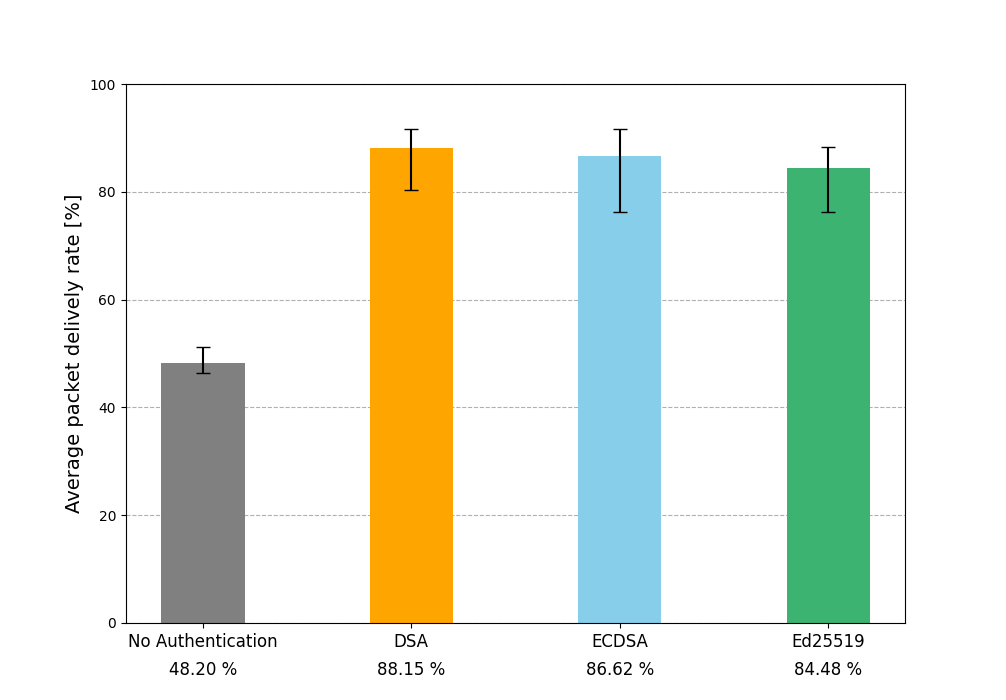
\includegraphics[width=1\textwidth]{figures/exp1_pdr.png}
  \caption{不正ノードが存在する環境でのパケット配送率}
  \label{fig:exp1_pdr}
\end{figure}
\clearpage
\begin{figure}
  \centering
  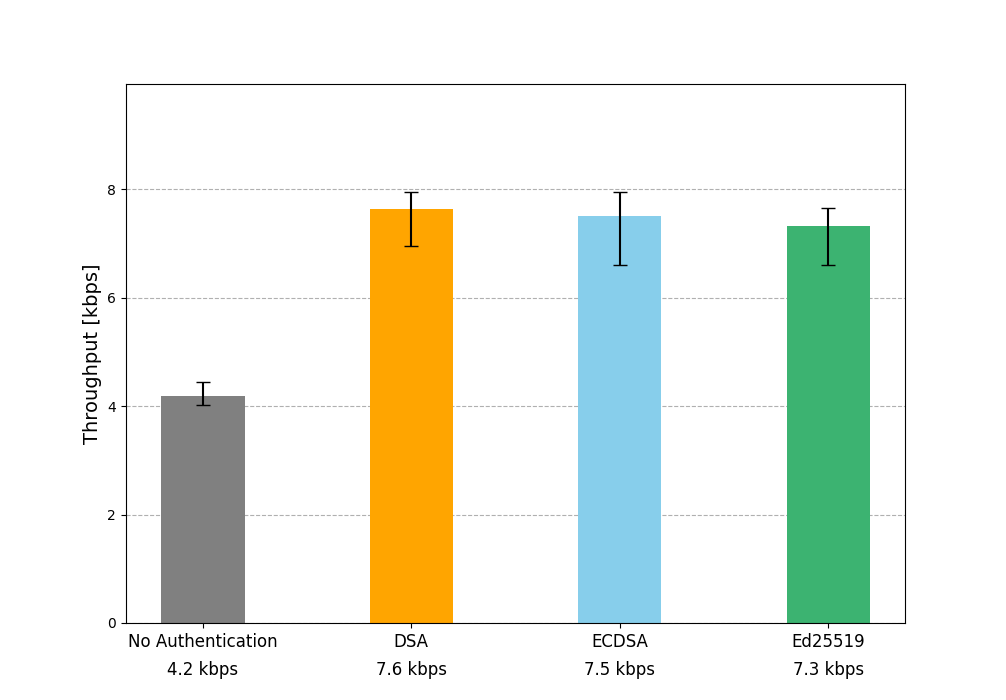
\includegraphics[width=1\textwidth]{figures/exp1_throughput.png}
  \caption{不正ノードが存在する環境でのスループット}
  \label{fig:exp1_throughput}
\end{figure}


\indent 図\ref{fig:exp1_pdr}は, 実験1におけるシミュレーションパターンごとの
パケット配送率を示している. 認証機構なしの場合に48.2 \%であるのに対し, 
ECDSAでは86.62 \%, EdDSAでは84.48 \%と, 認証機構を追加したことでパケット配送率が
約30 \%向上した. \\
\indent 図\ref{fig:exp1_throughput}は, 実験1におけるシミュレーションパターンごとの
スループットを示している. 認証機構なしの場合に4.18kbpsであるのに対し, 
ECDSAでは7.51kbps, EdDSAでは7.33kbpsと, 認証機構を
追加することでパケット配送率同様, スループットも向上した. \\
\indent これらの結果は, 認証機構の追加により 
不正ノードが排除されたことで, 経路選択を行う際に正当なノードのみが
選択されており,  データの窃取(転送中止)が回避できたことを示している. 
また, EdDSAの結果をECDSAの結果と比較するとほとんど差がないため, 
2つの署名方式が不正ノードを排除することにおいて同等のセキュリティ性能をもつと考えられる. 




\section{実験2}
実験2は認証機構の追加が通信にどれだけの負荷を与えるのかを
調査するための実験を行った. 
不正ノードの存在しない環境で, 250回シミュレーションを行い, 
遅延時間, 平均パケット配送率, オーバーヘッドサイズを調べた. \\
\indent 実験の結果は以下の通りである. \\

\begin{longtable}{ccc}
  \caption{遅延時間の中央値}
  \label{tab:exp2_delay} \\
  \endfirsthead
  \hline
  \multicolumn{1}{c}{プロトコル} &
  \multicolumn{1}{c}{中央値 [ms]} &
  \multicolumn{1}{c}{最頻値 [ms]} \\ \hline \hline
  No Authentication & $6.88$ & $[6.0, 7.0)$ \\
  DSA & $6.13$ & $[2.0, 3.0)$ \\
  ECDSA & $6.20$ & $[2.0, 3.0)$ \\
  Ed25519 & $6.42$ & $[6.0, 7.0)$ \\ \hline
\end{longtable}

\begin{figure}
  \centering
  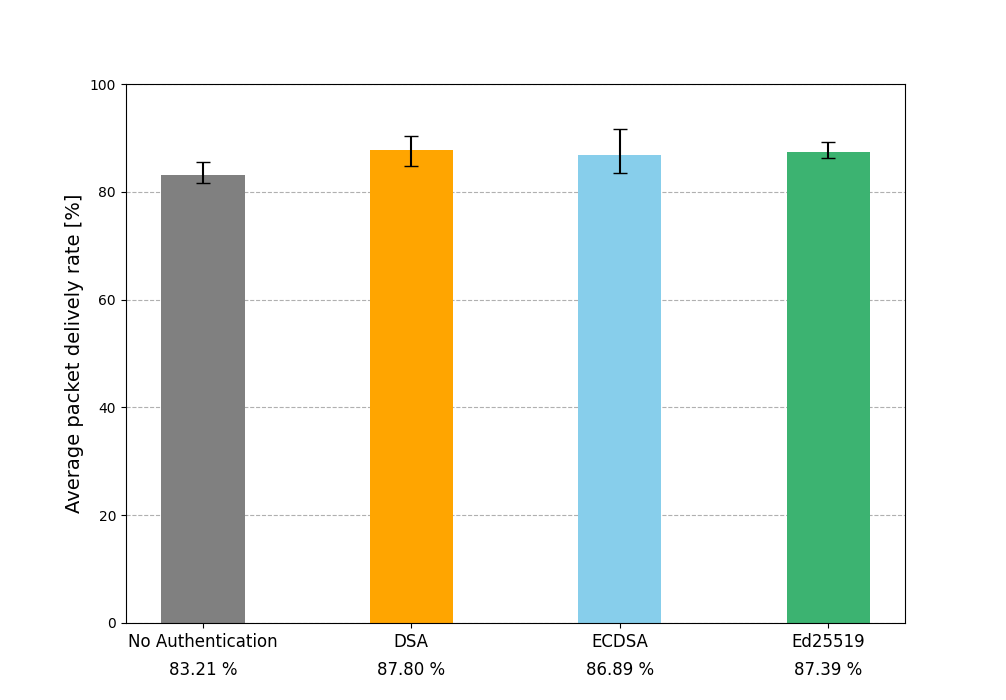
\includegraphics[width=1\textwidth]{figures/exp2_pdr.png}
  \caption{不正ノードが存在しない環境でのパケット配送率}
  \label{fig:exp2_pdr}
\end{figure}

\begin{figure}
  \centering
  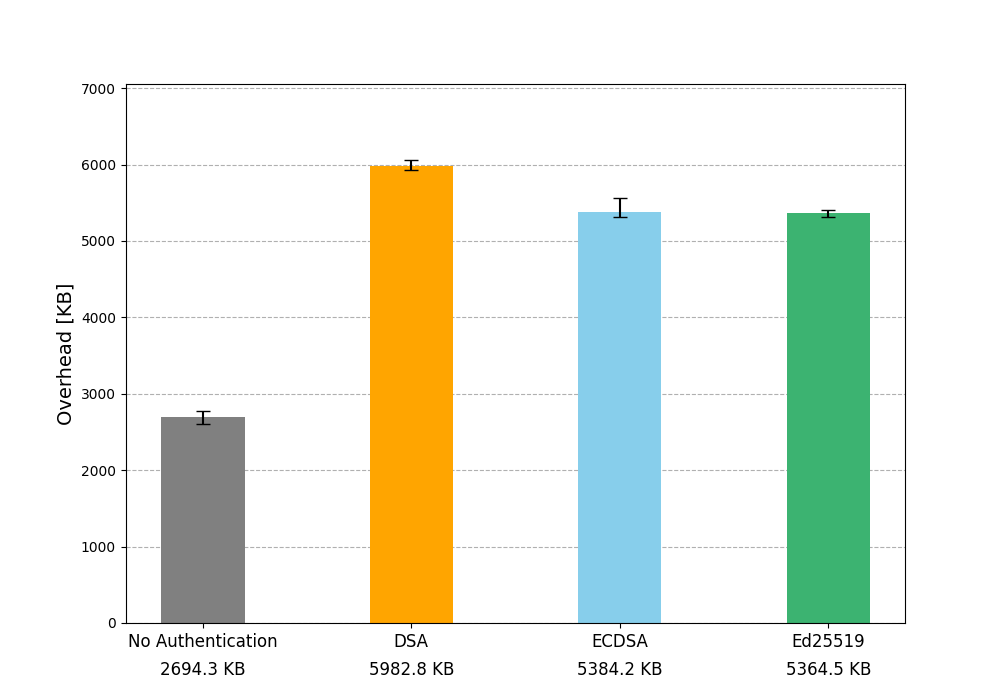
\includegraphics[width=1\textwidth]{figures/exp2_overhead.png}
  \caption{オーバーヘッドサイズ}
  \label{fig:exp2_overhead}
\end{figure}

\indent 表\ref{tab:exp2_delay}は, 実験2におけるシミュレーションパターンごとの
遅延時間の中央値と最頻値を示している. 中央値について, 認証機構なしでは6.88ms, 
DSAでは6.13ms, ECDSAでは6.2ms, EdDSAでは6.42msであった. 
最頻値について, 認証機構なしとEd25519では6.0msから7.0ms, 
DSAとECDSAでは2.0msから3.0msの範囲が最も多かった. 
この結果は, 遅延時間は経路選択のタイミングによって左右されるため, 
若干の差異が出てしまうが, 認証機構の有無が遅延時間に影響を与えなかったことを
示唆している. \\
\indent 図\ref{fig:exp2_pdr}は, 実験2におけるシミュレーションパターンごとの
平均パケット配送率を示している. 認証機構なしでは83.21 \%, DSAでは87.8 \%, 
ECDSAでは86.89 \%, EdDSAでは87.39 \%となった. この結果から, 
認証機構の有無はパケット配送率に影響を与えなかったと考えられる. \\
\indent 図\ref{fig:exp2_overhead}は, 実験2におけるシミュレーションパターンごとの
オーバーヘッドサイズを示している. 認証機構なしでは
2694.3KBであったのに対し, DSAでは5982.8KB, ECDSAでは5384.2KB, 
EdDSAでは5364.5KBと, 認証機構の追加により
オーバーヘッドサイズが大幅に増加した. これは, Helloパケットの
データに署名が付与されていることが原因である. また, 
EdDSAの結果をDSAとECDSAの結果と比較すると, EdDSAとDSAでは
大きな差があったのに対し, EdDSAとECDSAではほとんど差がなかった. 
EdDSAがDSAよりも鍵長が短いが, ECDSAとは変わらないことから
このような結果になったと考えられる. 
なお, 本研究で使用したパラメータによるそれぞれの鍵長は, 
DSAで2048ビット, ECDSAとEdDSAで256ビットである. \\



\section{実験3}
\indent 実験3では, 認証機構の処理能力(計算効率)を評価するための実験を行った. 
不正ノードの存在しない環境でノード数を37, 74, 112, 148, 185に設定して
250回ずつシミュレーションを行い, それぞれの実行にかかった時間を調べた.\\
\indent 実験の結果は以下の通りである. \\

\begin{figure}
  \centering
  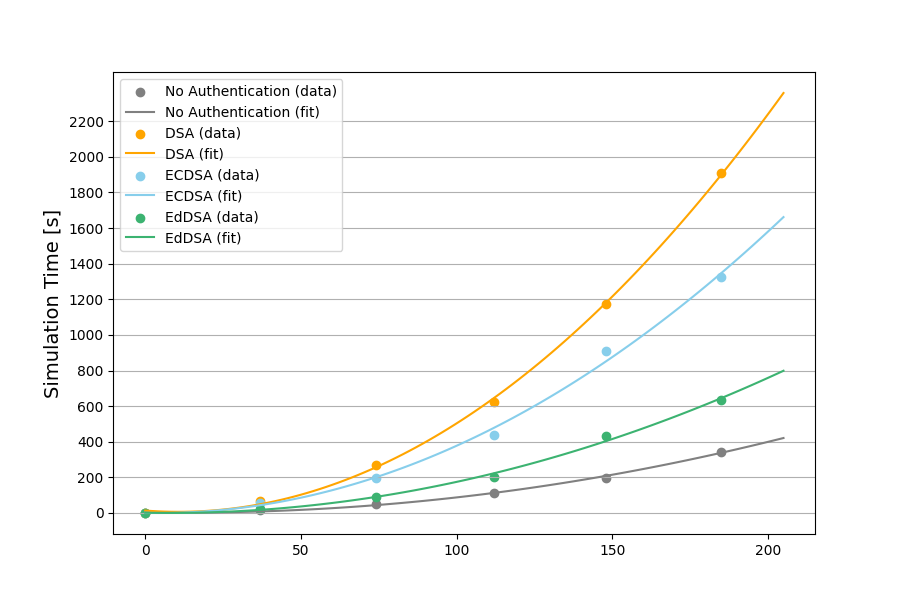
\includegraphics[width=1\textwidth]{figures/exp3_simtime.png}
  \caption{ノード数によるシミュレーション実行時間の変化}
  \label{fig:exp3_simtime}
\end{figure}

\setlength{\tabcolsep}{4pt}
\begin{longtable}{
    >{\raggedright\arraybackslash}p{3cm}
    >{\raggedright\arraybackslash}p{3.7cm}
    >{\raggedright\arraybackslash}p{2.5cm}
    >{\raggedright\arraybackslash}p{2.5cm}
    >{\raggedright\arraybackslash}p{2.5cm}
  }
  \caption{ノード数によるシミュレーション実行時間}
  \label{tab:exp3_simtime} \\
  \endfirsthead
  \hline
  % \multicolumn{1}{c}{Number of nodes} &
  % \multicolumn{1}{c}{No Authentication [s]} &
  % \multicolumn{1}{c}{DSA [s]} &
  % \multicolumn{1}{c}{ECDSA [s]} &
  % \multicolumn{1}{c}{Ed25519 [s]} \\ \hline \hline
  Number of nodes & No Authentication $[s]$ & DSA $[s]$ & ECDSA $[s]$ & Ed25519 $[s]$ \\ \hline \hline
  \multicolumn{1}{c}{$37$} &
  \multicolumn{1}{c}{$14.1802$} &
  \multicolumn{1}{l}{$69.9882$} &
  \multicolumn{1}{l}{$55.0108$} &
  \multicolumn{1}{l}{$24.4069$} \\
  \multicolumn{1}{c}{$74$} &
  \multicolumn{1}{c}{$50.5984$} &
  \multicolumn{1}{l}{$267.433$} &
  \multicolumn{1}{l}{$194.408$} &
  \multicolumn{1}{l}{$89.2728$} \\
  \multicolumn{1}{c}{$112$} &
  \multicolumn{1}{c}{$110.405$} &
  \multicolumn{1}{l}{$625.504$} &
  \multicolumn{1}{l}{$436.926$} &
  \multicolumn{1}{l}{$200.901$} \\
  \multicolumn{1}{c}{$148$} &
  \multicolumn{1}{c}{$196.971$} &
  \multicolumn{1}{l}{$1172.57$} &
  \multicolumn{1}{l}{$910.373$} &
  \multicolumn{1}{l}{$431.346$} \\
  \multicolumn{1}{c}{$185$} &
  \multicolumn{1}{c}{$345.059$} &
  \multicolumn{1}{l}{$1908.7$} &
  \multicolumn{1}{l}{$1324.55$} &
  \multicolumn{1}{l}{$635.155$} \\ \hline

  % $37$ & $14.1802$ & $69.9882$ & $55.0108$ & $24.4069$ \\
  % $74$ & $50.5984$ & $267.433$ & $194.408$ & $89.2728$ \\
  % $112$ & $110.405$ & $625.504$ & $436.926$ & $200.901$ \\
  % $148$ & $196.971$ & $1172.57$ & $910.373$ & $431.346$ \\
  % $185$ & $345.059$ & $1908.7$ & $1324.55$ & $635.155$ \\ \hline
\end{longtable}

\begin{longtable}{ccc}
  \caption{1回の署名作成と署名検証にかかった時間}
  \label{tab:exp3_sigtime} \\
  \endfirsthead
  \hline
  \multicolumn{1}{c}{プロトコル} &
  \multicolumn{1}{c}{署名作成時間 $[\mu s]$} &
  \multicolumn{1}{c}{署名検証時間 $[\mu s]$} \\ \hline \hline
  ECDSA & $371.020$ & $336.938$ \\
  Ed25519 & $31.349$ & $97.036$ \\ \hline
\end{longtable}

\indent 図\ref{fig:exp3_simtime}はシミュレーションパターンごとのノード数による
実行時間の変化を近似してグラフ化したものを, 表\ref{tab:exp3_simtime}はその具体的な
値を示したものである. さらに, 表\ref{tab:exp3_sigtime}にはECDSAとEdDSAにおいて, 1回の署名作成と
署名検証にかかった時間を示した. \\
\indent 図\ref{fig:exp3_simtime}, 表\ref{tab:exp3_sigtime}より, 
EdDSA, ECDSA, DSAの順番で実行時間が短いのがわかる. また, 
表\ref{tab:exp3_sigtime}に示すように, EdDSAがECDSAに比べて
署名生成, 署名検証にかかる時間が短いことから, EdDSAは
3つの署名方式の中で最も計算効率が良いということが確かめられた. 
さらに, ECDSAとEdDSAの計算効率の差はノード数が増加するほど, 
実行時間全体に与える影響が大きなっており, EdDSAが
よりスケーラビリティに優れていることを示唆している. 
\chapter[   EdDSAに関する実装評価まとめ]{EdDSAに関する実装評価まとめ}
この章では, 2章で説明したEdDSAの性能と5章で示した実験結果から, 
EdDSAの実装評価をする. はじめに, 5章で示した実験結果の評価を
他の認証方式と比較しながらまとめ, その後に2章の内容を含めながら
ECDSAとの総合的な比較評価を行う. 最後に, 本研究で行った実験結果から
想定されるEdDSAの利用シーンについて考察する.\\[1em]
\noindent {\large\textbf{実験結果のまとめ}} 
\begin{enumerate}
  \item 実験1\\
  \indent EdDSAを用いたことで, 不正ノードを排除することができたが, 
  他の認証方式との差は見られなかった. 
  \item 実験2\\
  \indent 平均遅延と平均パケット配送率において, EdDSAは他の
  認証方式との差は見られなかったが, それぞれの鍵長の違いから
  オーバーヘッドサイズがDSAよりも小さく, ECDSAと同程度であった.
  \item 実験3\\
  \indent EdDSAは他の認証方式よりも署名の生成と検証にかかる時間が
  短いことから, 処理能力(計算効率)が高いことがわかった.
\end{enumerate}

\noindent {\large\textbf{EdDSAとECDSAの比較評価}}\\
\indent 上記の実験結果のまとめから, EdDSAはECDSAよりも
計算効率が高いことがわかった. これは, 第2章で述べたEdDSAの設計上の
特長である高速な処理能力が実験環境においても十分に発揮されたことを
示している. また, 第2章で述べたセキュリティの堅牢性から, 
EdDSAは秘密鍵を特定しようとする攻撃者が存在する環境でECDSAよりも
高いセキュリティを提供できる. よって, V2Vアドホックネットワーク
において, EdDSAはECDSAよりも安全かつ効率的な認証方式として
利用できるといえる.\\

\noindent {\large\textbf{EdDSAの利用シーンについての考察}}\\
\indent シミュレーション実験からEdDSAは他の認証方式, 特にECDSAと比べても
通信品質が向上, または同等であることがわかった. さらに, 実験2で採取したデータに
メモリ使用量がある. 図\ref{fig:memory_usages}に示すように,   
Ed25519のメモリの使用量がECDSAよりも少ないことがわかる. 
また, 本研究の実験環境では, EdDSAの署名の生成と検証の時間が
データパケットとHelloパケットの送信間隔(1秒)に比べて非常に短いということから, 
次のような環境であれば署名の生成と検証の回数がより多くなり, 
EdDSAの処理効率を最大限に発揮できると考えられる. 
\begin{itemize}
  \item ノード数が非常に多い
  \item データパケットとHelloパケットの送信間隔が非常に短い
  \item 使えるリソースが限られている
\end{itemize}
さらに, 次のような環境であればEdDSAのセキュリティの堅牢さを
発揮すると考えられる. 
\begin{itemize}
  \item 秘密鍵を特定しようとする攻撃者が存在する
\end{itemize} 
% \par\indent 以上のことから, EdDSAはV2VアドホックネットワークやIoT
% が発展していく中で, 今後ますます重要な役割を果たすと考えられる.\\

\begin{figure}
  \centering
  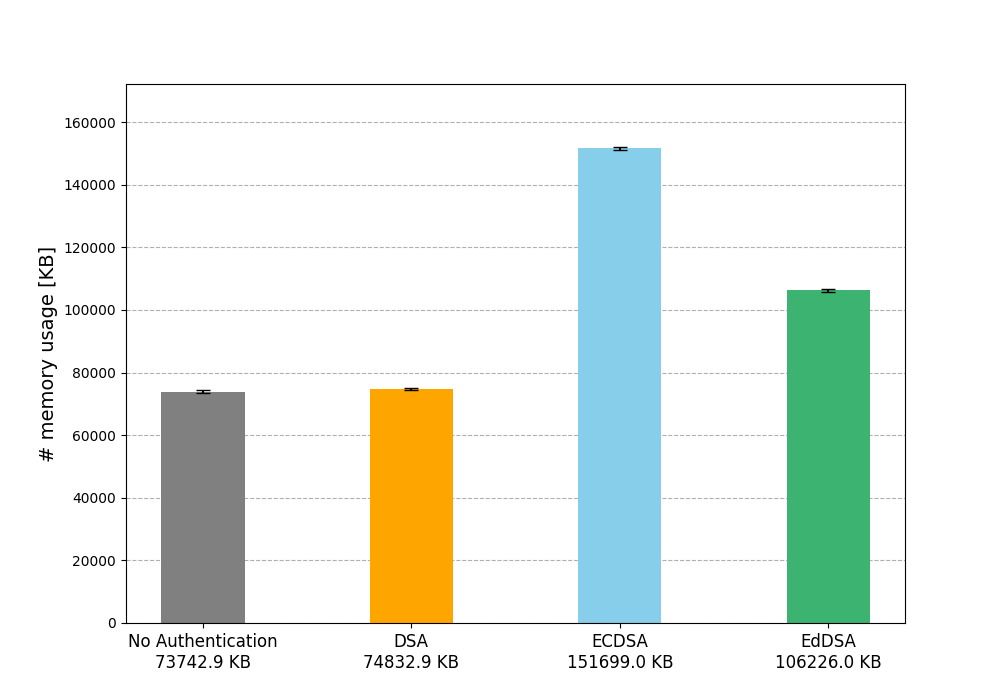
\includegraphics[width=1\textwidth]{figures/memory_usages.png}
  \caption{メモリ使用量}
  \label{fig:memory_usages}
\end{figure}







\chapter*{おわりに}
\addcontentsline{toc}{chapter}{おわりに}  % 目次に追加
本論文は6章で構成される. 第1章では, VANETやデジタル署名について
説明した. 第2章では, 本研究の対象であるEdDSA(Ed25519)の特徴や
アルゴリズムについて解説した. 第3章では, セキュアに
ルーティングを行うためにの認証機構の導入方法について解説した. 
第4章では, シミュレーション環境について述べ, 第5章で
シミュレーションによる実験を行い, その結果と評価を示した. 
第6章では, 第2章と第5章の内容を踏まえ, EdDSAの実装評価について議論した. \\
\indent 本研究では, EdDSAの高い計算効率および堅牢なセキュリティ性能が, 
認証機構を追加したGPSRによるV2V通信にどのような影響を与えるかを
検証した. その結果, EdDSAを使用した場合, 署名生成および
検証にかかる処理時間が他の署名方式(ECDSA, DSA)よりも短縮され, 
ネットワーク全体の計算負荷が軽減されることを明らかにした. 
また, EdDSAの性能を最大限活かすための利用シーンの考察すると, 
EdDSAはV2VアドホックネットワークやIoTが発展に伴い, 
今後ますます重要な役割を果たすと考えられる.\\
\chapter*{謝辞}
\addcontentsline{toc}{chapter}{謝辞}  % 目次に追加
本論文は筆者である永野が岐阜大学工学部電気電子・情報工学科情報コースに
在籍中の研究成果をまとめたものです. 本研究は多くの方々のご指導, 
ご協力のもと行われており, その方々の助力なくして, 
本研究は成立しませんでした. ここに深く感謝申し上げます. \\
\indent 筆者の指導教員である三嶋美和子教授および角田有助教には, 
研究の理論的な基盤の構築からその詳細な検討, 執筆活動にわたるまで, 
多くの助言と細やかなご指導をいただきました. 
ここに心から感謝の意を表します. \\
\indent また, 岐阜大学工学部フェロー原山美知子先生には, 
本研究における実践的な技術の整理や考察に関して, 的確な
アドバイスを数多くいただきました. 原山先生のご助言は, 
本研究の完成度を高める上で欠かせないものでした. 深く感謝申し上げます.\\ 
\indent 最後に, 本研究を遂行するにあたり, 三嶋研究室の皆様には
多大なご協力をいただきました. 苦楽を共にした同窓生である
大野氏, 野田氏, 加藤氏の3人に, 感謝いたします.\\[5em]

\begin{flushright}
  令和7年2月5日\\
  岐阜大学工学部電気電子・情報工学科情報コース\\
  永野 正剛
\end{flushright}
  
\chapter*{参考文献}
\addcontentsline{toc}{chapter}{参考文献}  % 目次に追加
\bibliographystyle{junsrt}
\bibliography{references}

\end{document}